\section{Design Evaluation}

\subsection{Virtual Mesh Network Simulation}
\label{sec:virtual_mesh_simulation}

In addition to using the Coracle simulator, we also developed a virtual mesh network simulator that interfaces with our software implementation to run rapid simulations and obtain readable logs for debugging and testing. The simulator also enables us to deploy our library implementation code to a large number of nodes, such as 100+ nodes, in a few seconds without actually buying the required hardware.

Our simulator directly runs our library implementation code without any modifications. The simulator virtualizes required resources such as the network card, serial input/output, and other dependent software libraries in order to provide an identical environment to the ESP8266 microcontroller, as shown in Figure \ref{fig:virtual_esp_diagram}. The simulation loads our library implementation code to virtual nodes in the simulated environment and manages the networking between these virtual nodes. As a result, we are able to control which nodes connect to each other and simulate various network conditions such as missing links. We are also able to add or remove new virtual nodes to the system and observe how the entire network behaves.

Furthermore, the simulator allows us to reliably collect metrics about our software implementation and learn how they change depending on parameters, such as the number of nodes in the network.


\begin{figure}[H]
    \centering
    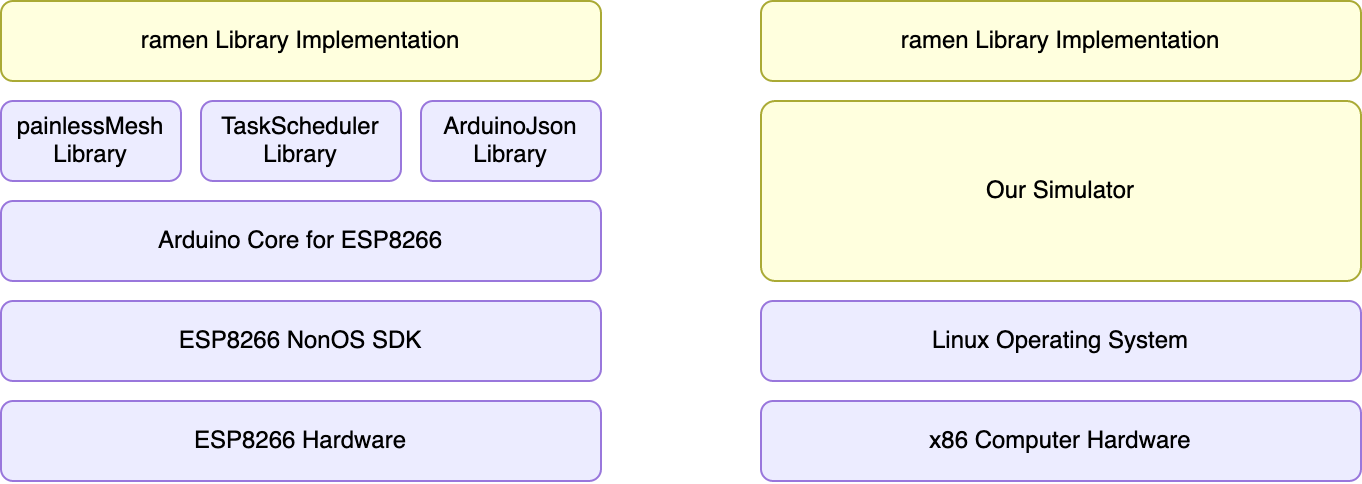
\includegraphics[width=0.85\columnwidth]{images/virtual_esp.png}
    \caption{Left: Our software implementation running on ESP8266 hardware, Right: Our software implementation running on our simulator }
    \label{fig:virtual_esp_diagram}
\end{figure}


\subsection{Criteria for Testing}

To evaluate our implementation of Raft, we have selected three main criteria: network scalability, network stability, and network realignment time. We first conducted experiments in the Coracle simulation to obtain a baseline. We then conducted the experiments in the virtual mesh simulation to test how our implementation compared.

\begin{itemize}
    \item \textit{Network scalability:}
    \begin{itemize}
        \item Network scalability refers to how well the network performs with various densities of nodes. Increasing the number of nodes should not significantly increase latency.
    \end{itemize}

    \item \textit{Network stability:}
    \begin{itemize}
        \item Network stability implies that the network should perform reliably and consistently over time so as to avoid any loss of data. 
    \end{itemize}
    
    \item \textit{Realignment time:}
    \begin{itemize}
        \item Realignment time measures the network's ability to recover from abrupt changes to the system, such as the loss of a leader.
    \end{itemize}
\end{itemize}



\subsection{Test Data}

Each simulation shown in Figures \ref{fig:virtual_vary_nodes}, \ref{fig:virtual_vary_duration}, \ref{fig:virtual_vary_heartbeat}, \ref{fig:virtual_vary_election_timeout}, and \ref{fig:virtual_vary_leader_kill} was run for 60 seconds in the virtual mesh network simulator using our ramen library. Each of the simulations shown in Figures \ref{fig:virtual_vary_duration}, \ref{fig:virtual_vary_heartbeat}, and \ref{fig:virtual_vary_election_timeout} were run with 5 nodes per run.

\subsubsection{Measurements}

\begin{figure}[H]
    \centering
    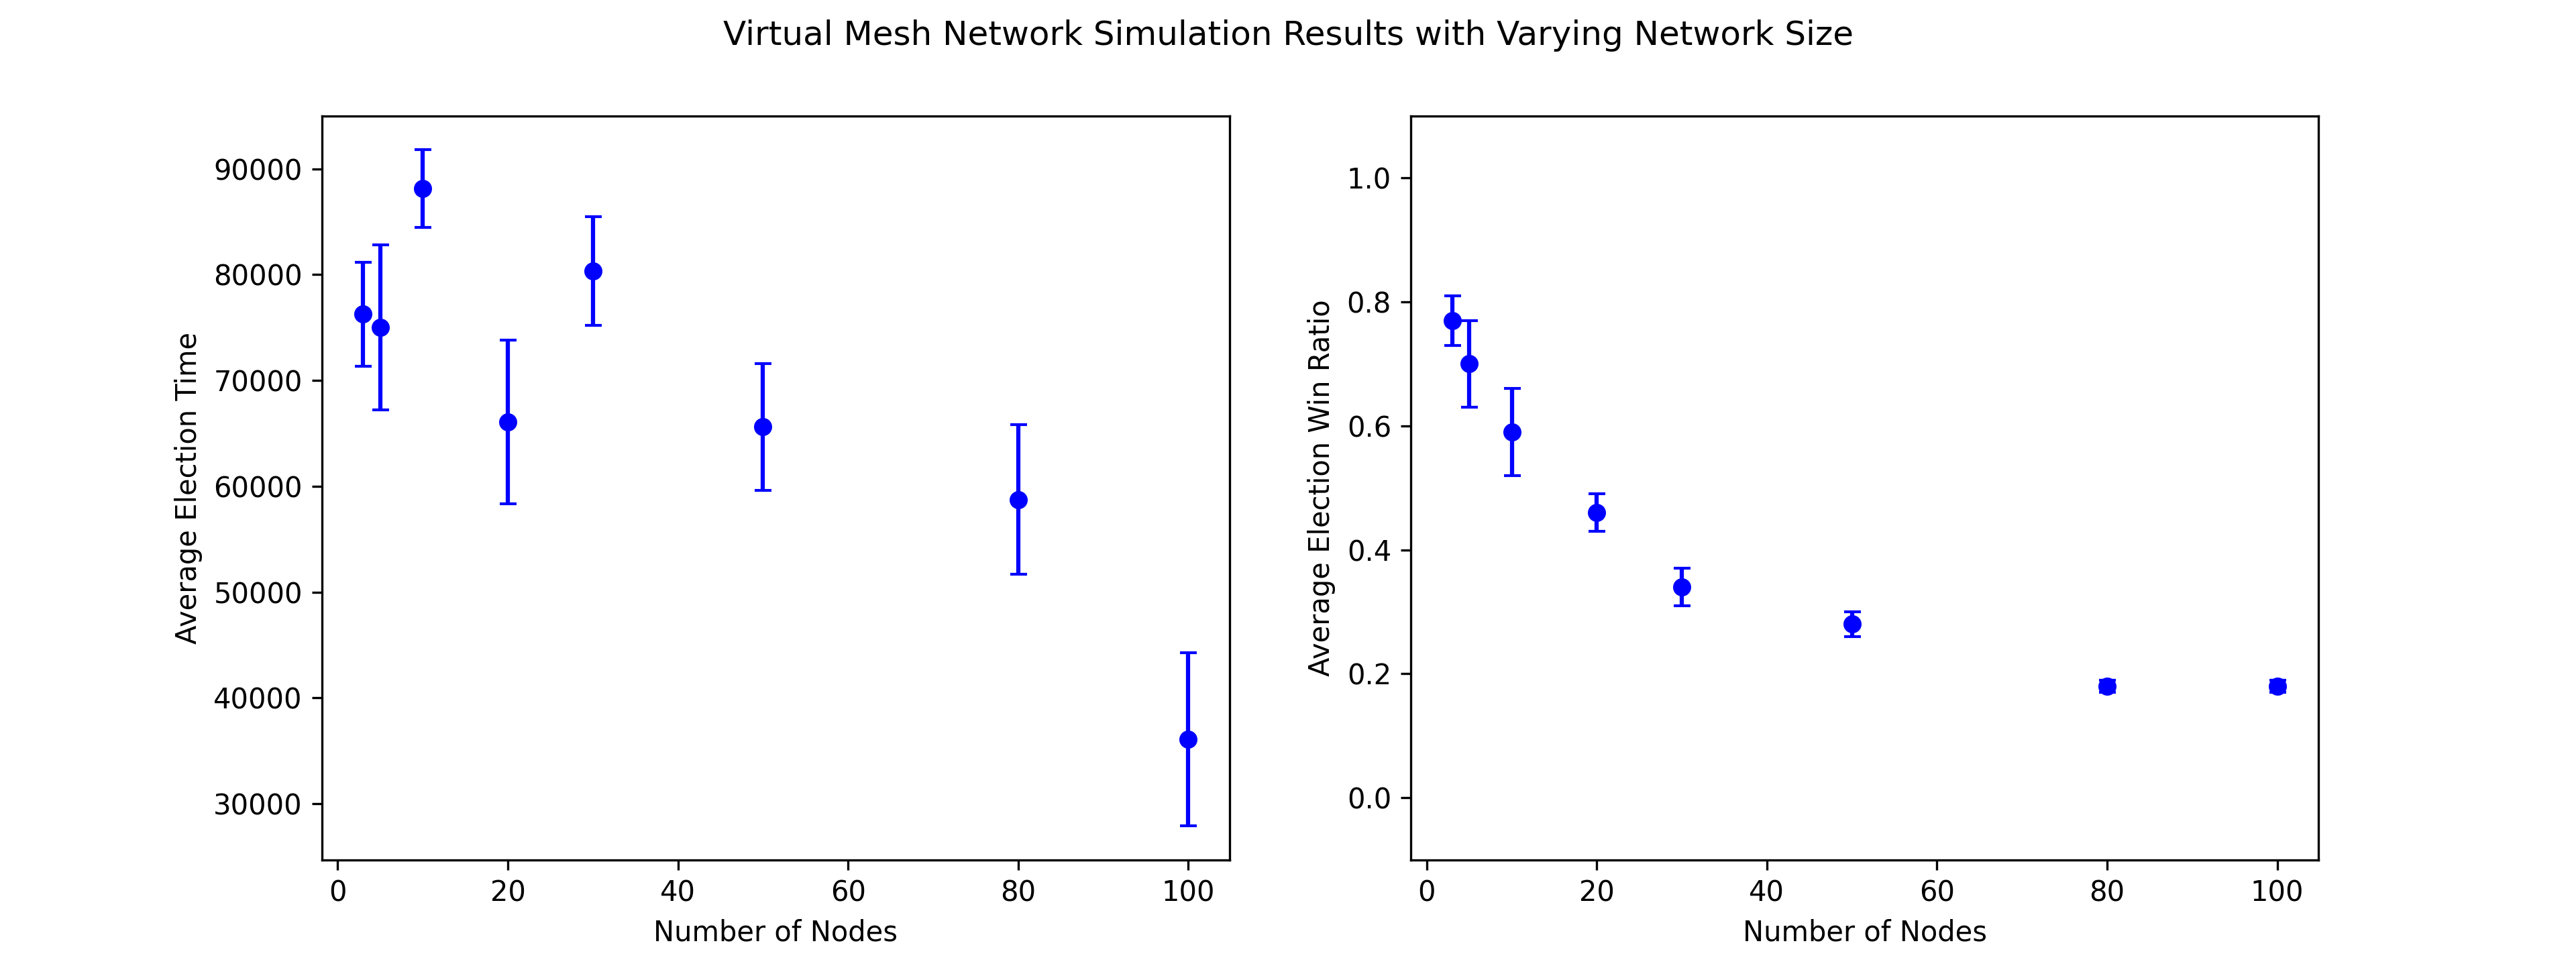
\includegraphics[width=0.9\columnwidth]{images/virtual_vary_nodes.png}
    \caption{Left: Average election time per number of nodes, Right: Average ratio of elections won to initiated per number of nodes}
    \label{fig:virtual_vary_nodes}
\end{figure}


\begin{figure}[H]
    \centering
    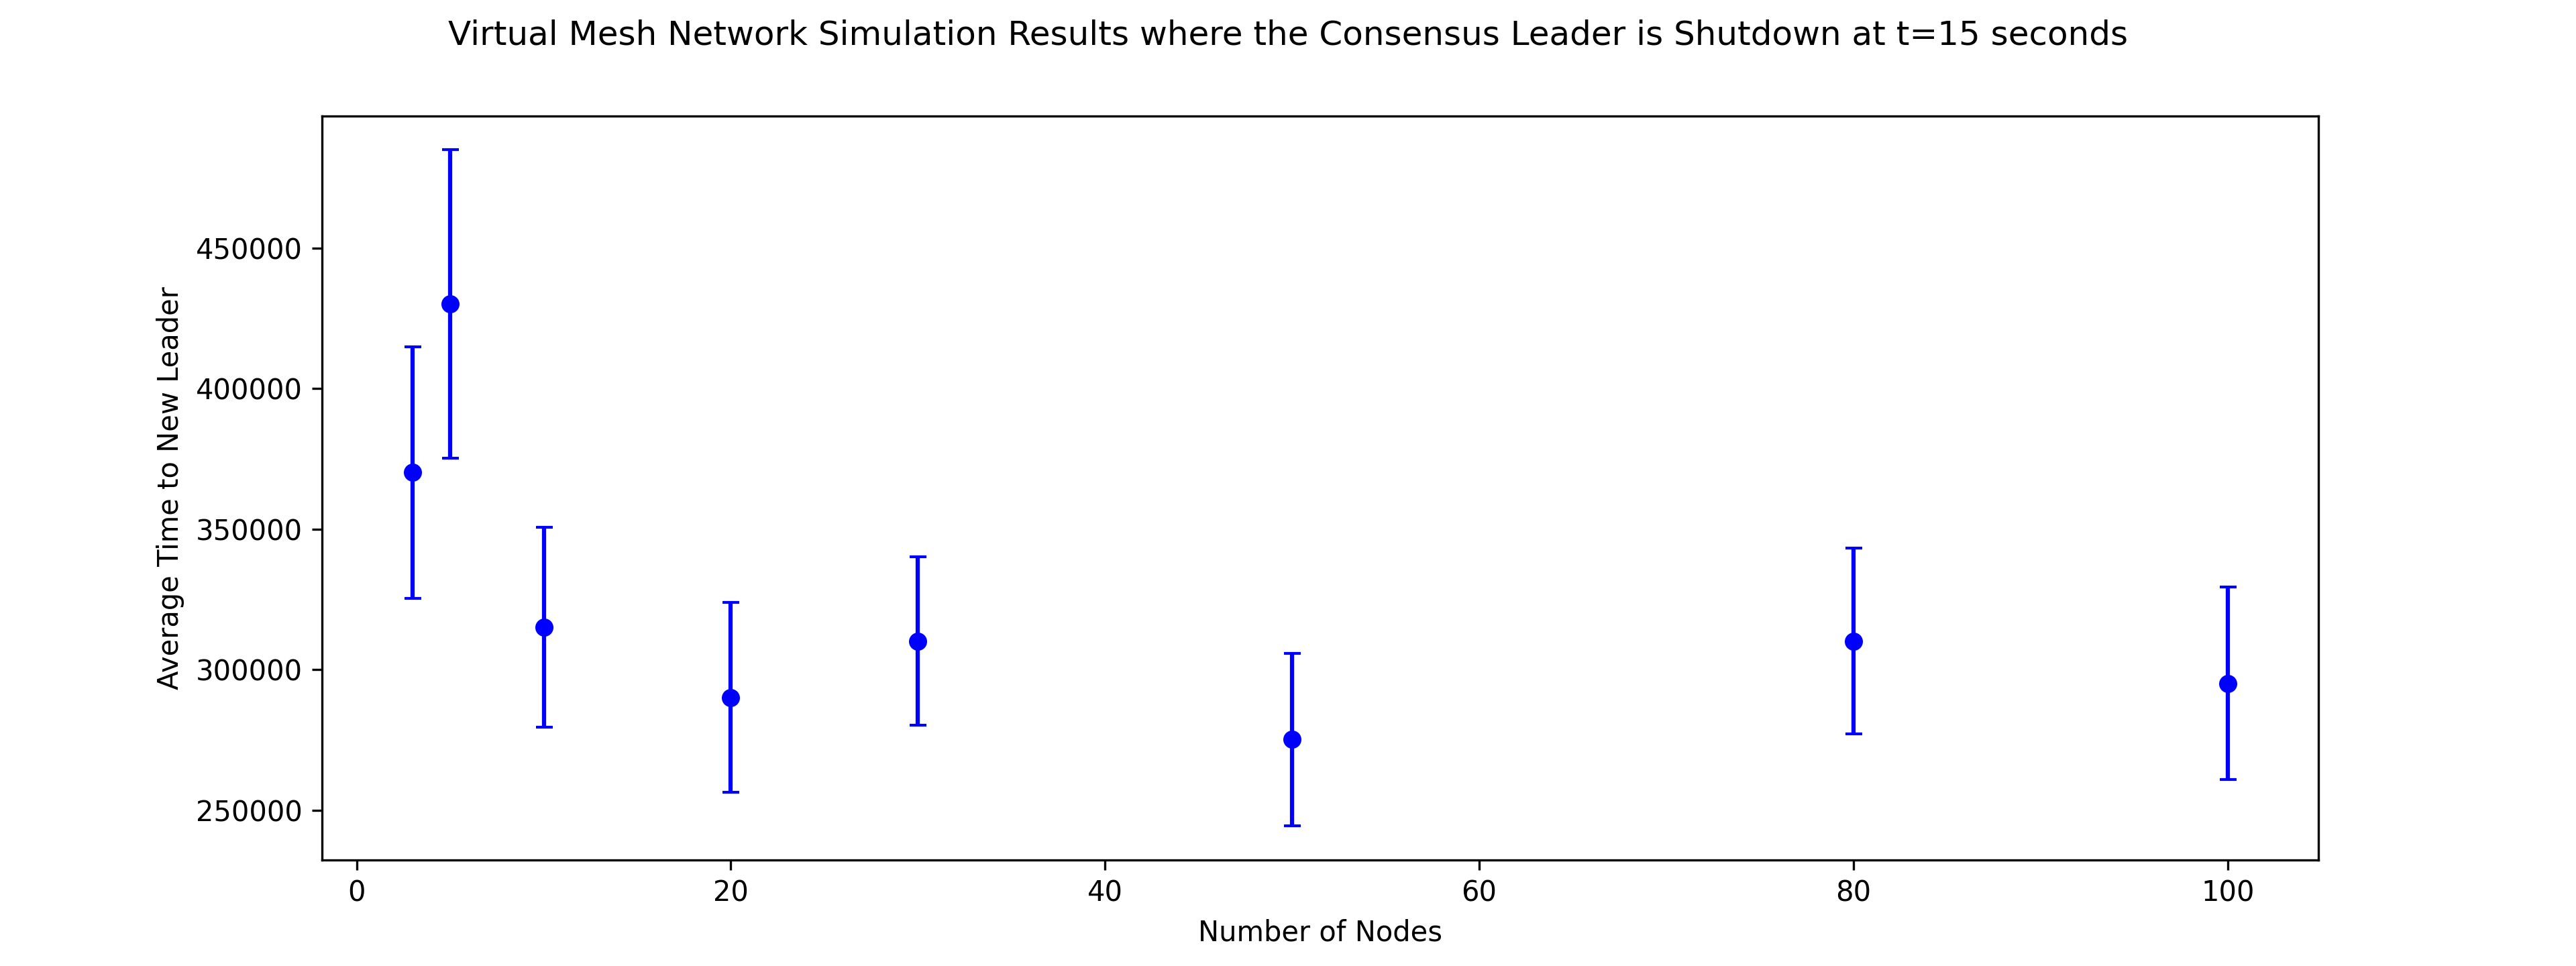
\includegraphics[width=0.9\columnwidth]{images/virtual_vary_leader_kill.png}
    \caption{Average time to elect new leader per number of nodes when the leader is shutdown}
    \label{fig:virtual_vary_leader_kill}
\end{figure}


\begin{figure}[H]
    \centering
    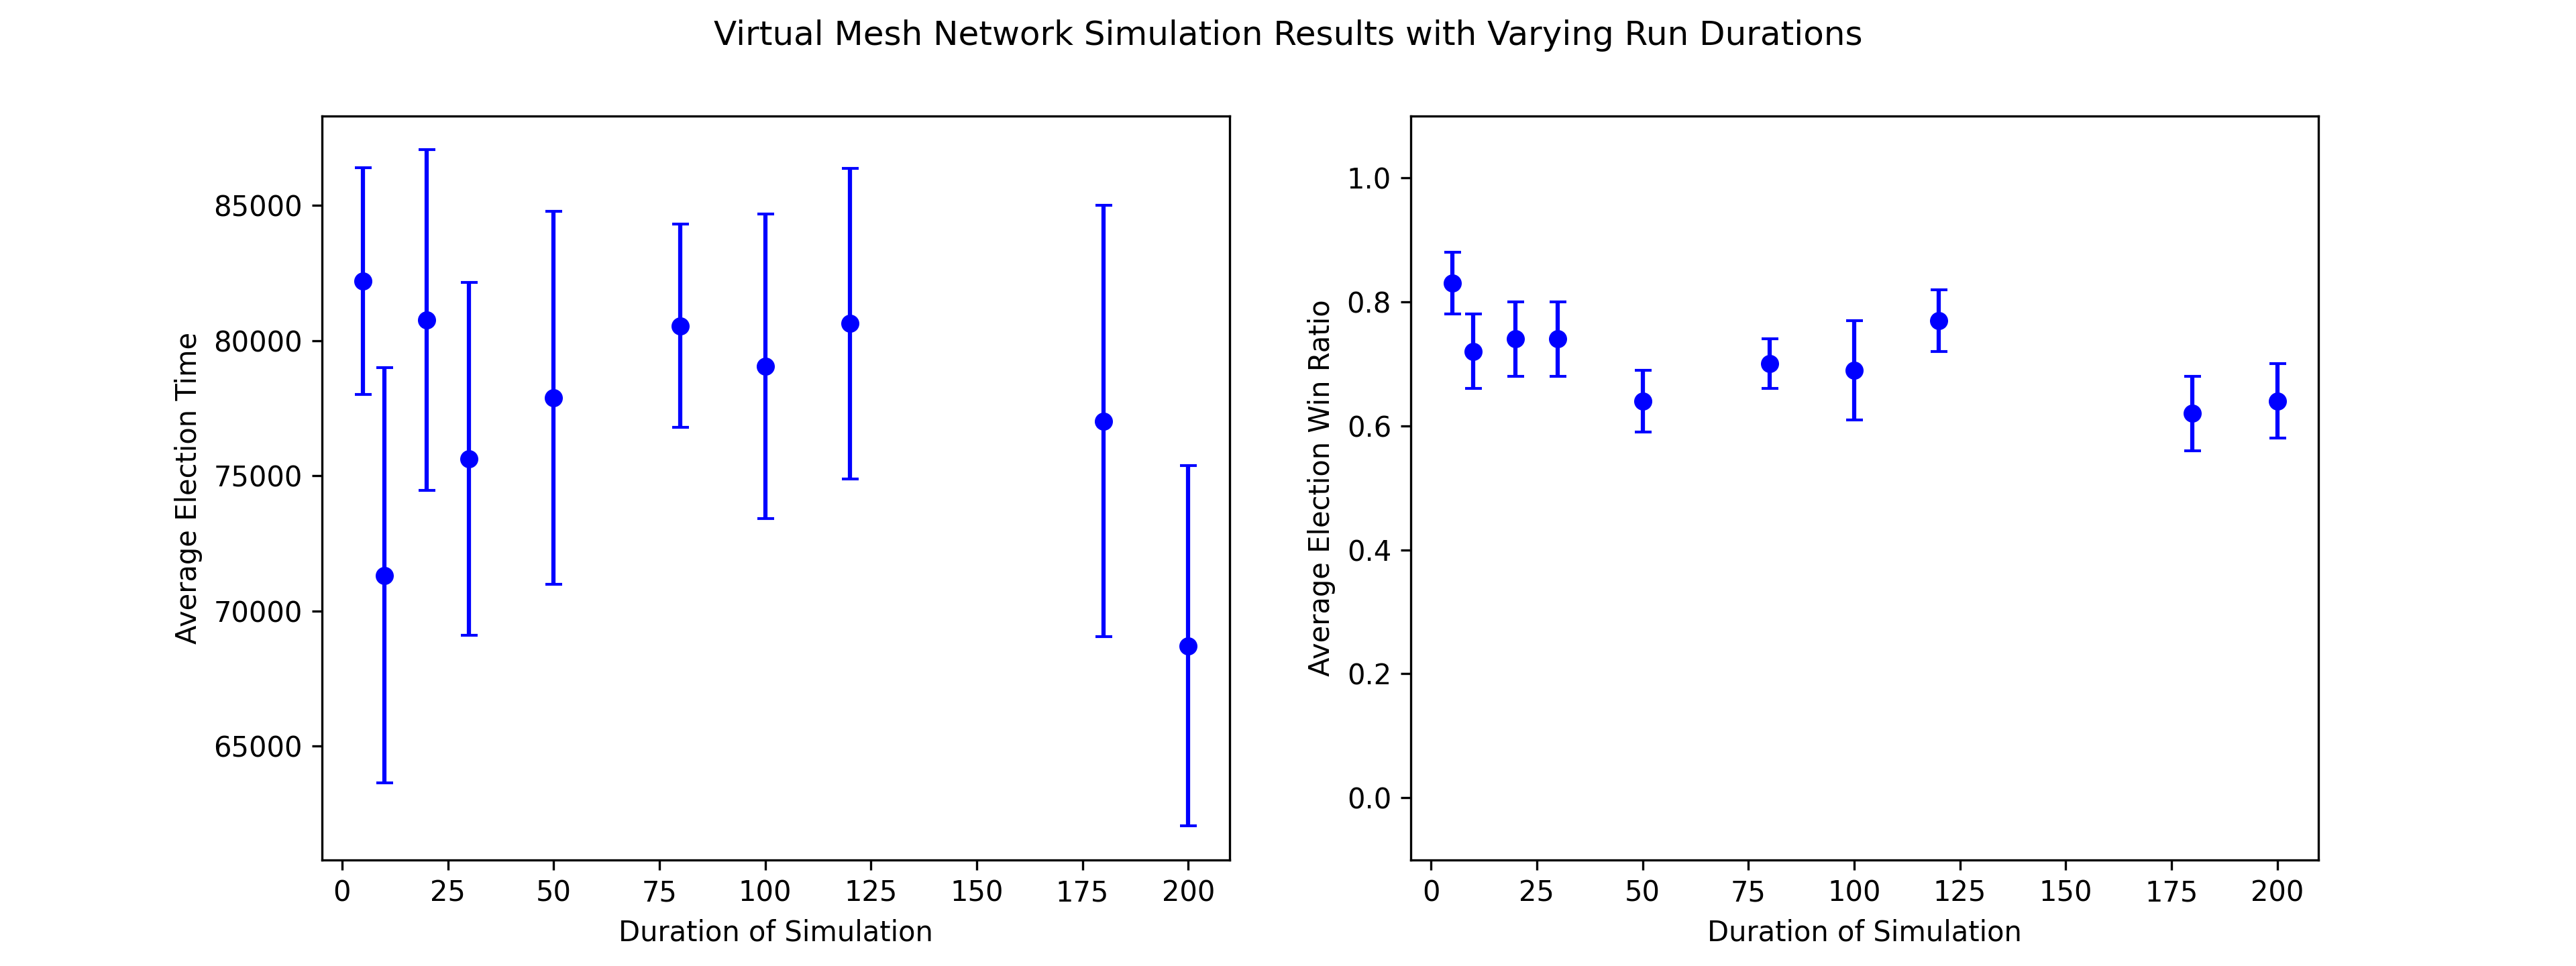
\includegraphics[width=0.9\columnwidth]{images/virtual_vary_duration.png}
    \caption{Left:Average election time per change in simulation run duration, Right: Average ratio of elections won to initiated per change in simulation run duration}
    \label{fig:virtual_vary_duration}
\end{figure}


\begin{figure}[H]
    \centering
    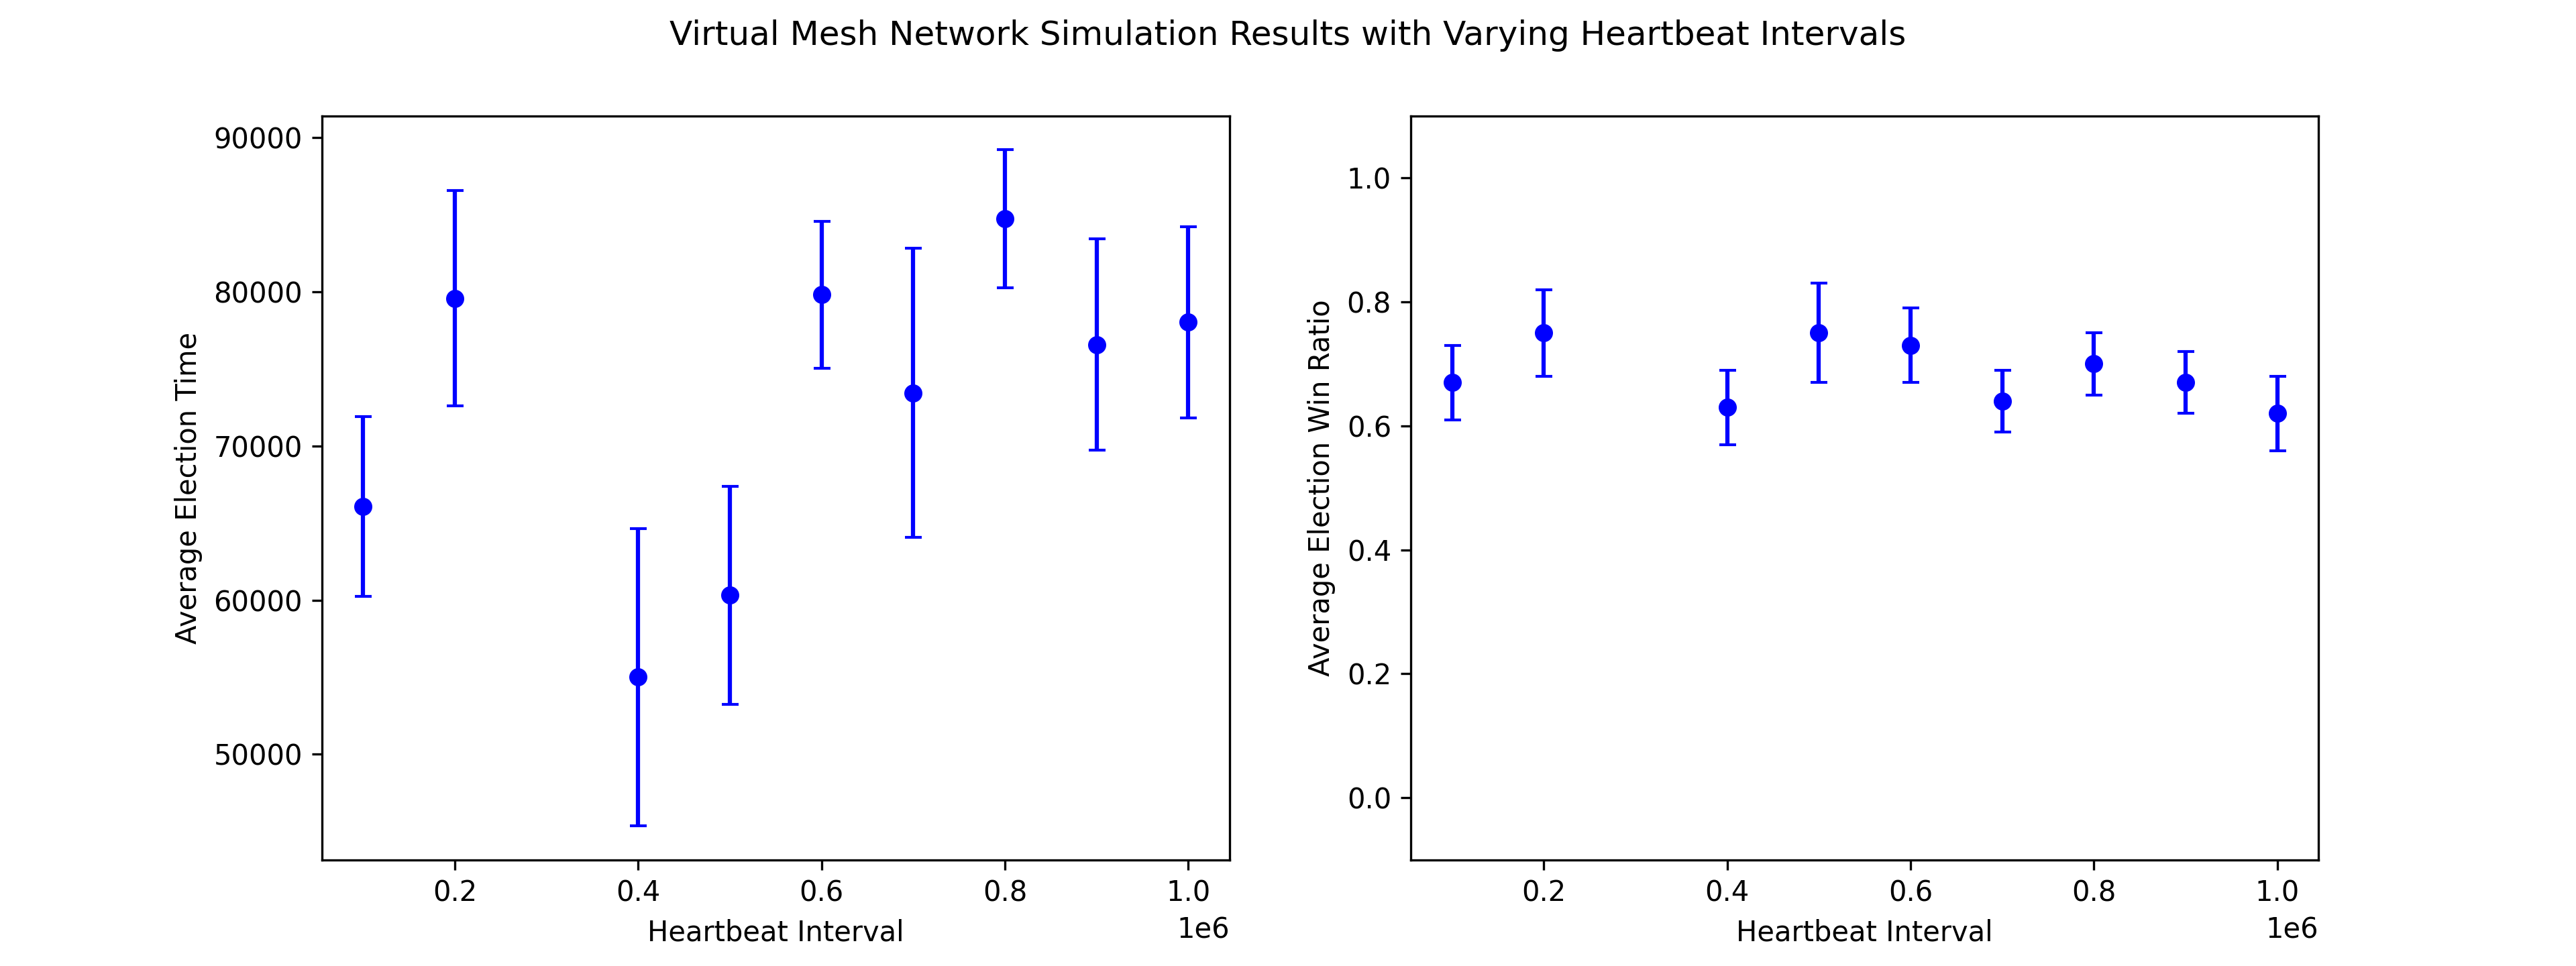
\includegraphics[width=0.9\columnwidth]{images/virtual_vary_heartbeat.png}
    \caption{Left: Average election time per change in heartbeat interval, Right: Average ratio of elections won to initiated per change in heartbeat interval}
    \label{fig:virtual_vary_heartbeat}
\end{figure}


\begin{figure}[H]
    \centering
    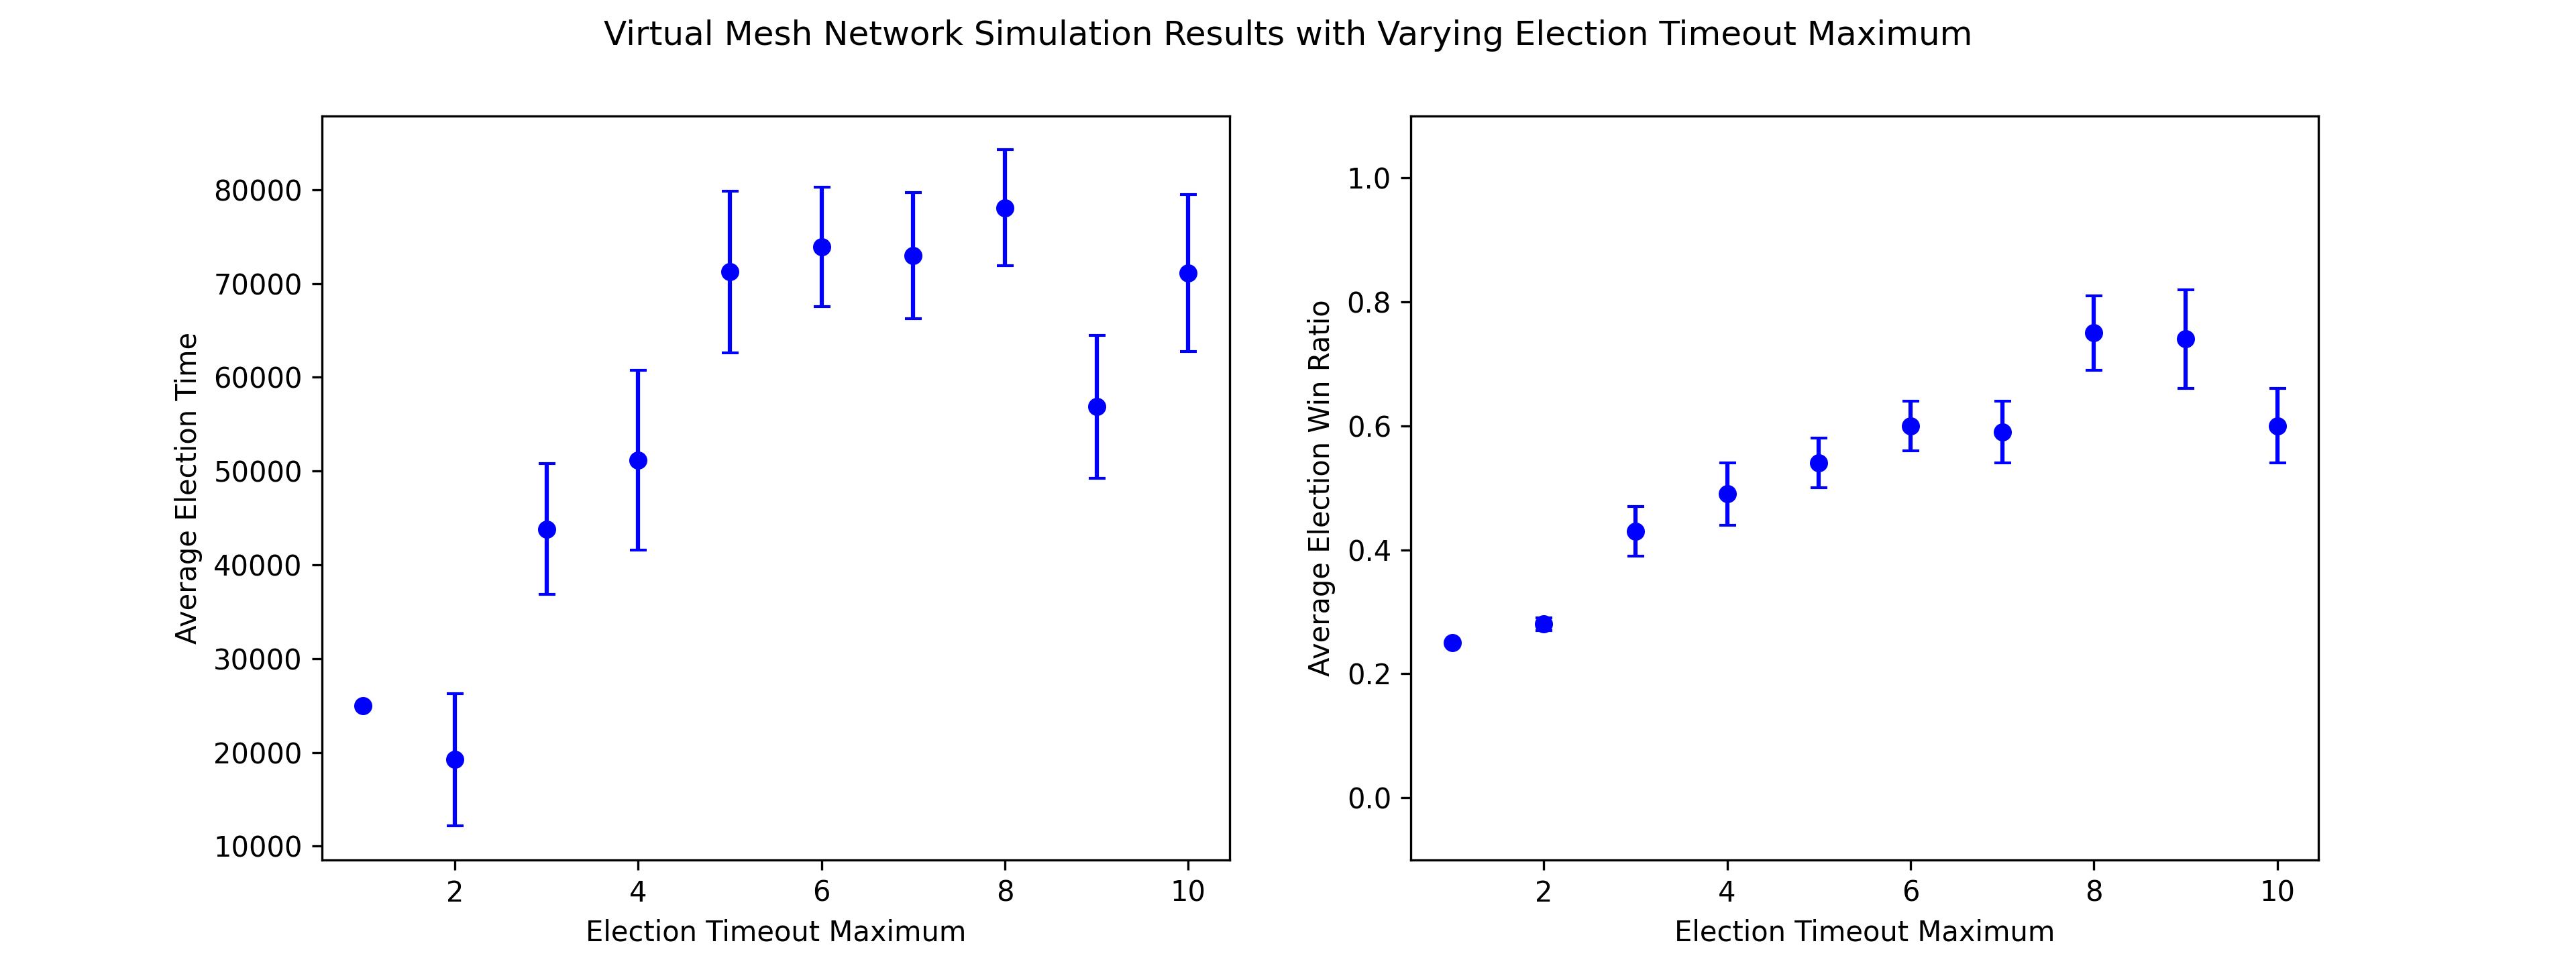
\includegraphics[width=0.9\columnwidth]{images/virtual_vary_election_timeout.png}
    \caption{Left:Average election time per change in maximum possible election timeout, Right: Average ratio of elections won to initiated per change in maximum possible election timeout}
    \label{fig:virtual_vary_election_timeout}
\end{figure}


\subsubsection{Meeting the Specifications}

\begin{table}[H]
    \centering
    \footnotesize
    \renewcommand{\arraystretch}{2.5}
    \vspace{10pt}
    \caption{Meeting the testing criteria and design constraints of the capstone project}
    \label{tab:meeting_the_specificatons}
    \begin{tabular}{|l|p{5cm}|p{5cm}|}
        \hline
        \textbf{Testing Criterion}   & \textbf{Specifications} & \textbf{Meeting the Specifications} \\ 
        \thickhline 
        Resilient to threats  & The network should recovering from the loss of a consensus leader within 1000\si{\ms} & In average it takes 300 \si{\ms} for a new leader to be elected after a failure as shown in Figure \ref{fig:virtual_vary_leader_kill}. \\ \hline
        Scalability           & The network should support at least 100 nodes in an area covering 1000\si{m^2} & The network can support more than 100 nodes.  \\ \hline
        Low power consumption & The board should consume below 100\si{mA} on average use while running the library & The board consumes 91\si{mA} on average use while running the library. \\ \hline
        Small footprint       & The compiled library should fit into an embedded 2\si{MB} flash memory. & The compiled code takes up  0.33\si{MB} of space in the flash memory. \\ \hline
    \end{tabular}
\end{table}


\subsection{Discussion}

We were able to successfully implement the Raft consensus algorithm for embedded systems atop a mesh network. The measured performance of our software library complements the results we obtained from our modeling and Coracle simulation results. Figure \ref{fig:virtual_vary_nodes} shows that there is not a drastic drop in performance as the network size increases; the decrease and eventual plateau in the election win to started ratio are expected and on par with our simulations, as shown in Figure \ref{fig:coracle_vary_nodes}. Figure \ref{fig:virtual_vary_leader_kill} shows the results of shutting down the consensus leader halfway through the simulation and measuring the time it takes to re-elect a new leader. We see that as the network size grows, the time to re-election is not significantly affected. Furthermore, in Figure \ref{fig:virtual_vary_election_timeout}, the results seem to indicate that the optimal maximum election timeout lies between 8-9 seconds.  Otherwise, the graphs show a similar trend to the Coracle simulations, where a greater average timeout maximum leads to a greater average election time and a greater average election win ratio.

Changing the run duration of the simulation and changing the heartbeat interval does not seem to have a significant effect on the system, as evidenced by the large standard error bars in Figure \ref{fig:virtual_vary_duration} and \ref{fig:virtual_vary_heartbeat}. These results are expected: running the simulation longer with no significant difference implies that the network remains stable while increasing the heartbeat interval should not have an impact on the elections. 

Therefore, overall, the obtained results suggest that our implementation meets the design requirements for creating a resilient mesh network coupled with a consensus algorithm.